%Title:  What has been tried for system 8 and what is example.
 
\documentclass[11pt]{article}
\usepackage{amssymb,latexsym,amsmath}
\usepackage{graphicx}
\usepackage{epsfig}
\usepackage{enumerate}
\usepackage[top=1in,right=1in,left=1in,bottom=1in]{geometry}

%-----------------------------------------------------------------
\vfuzz2pt % Don't report over-full v-boxes if over-edge is small
\hfuzz2pt % Don't report over-full h-boxes if over-edge is small
% THEOREMS -------------------------------------------------------
%\theoremstyle{remark}
%\newtheorem*{rem}{Remark}
% MATH -----------------------------------------------------------
\newcommand{\abs}[1]{\left\vert#1\right\vert}
\newcommand{\set}[1]{\left\{#1\right\}}
\newcommand{\Real}{\mathbb R}
\newcommand{\Z}{\mathbb Z}
\newcommand{\Q}{\mathbb Q}
\newcommand{\To}{\rightarrow}
\newcommand{\display}[1]{\begin{displaystyle}#1\end{displaystyle}}
\renewcommand{\phi}{\varphi}
%\newtheorem{theorem}{Theorem}[section]
%\newtheorem{lemma}[theorem]{Lemma}
%\newtheorem{proposition}[theorem]{Proposition}
%\newtheorem{corollary}[theorem]{Corollary}

\newenvironment{proof}[1][Proof]{\begin{trivlist}
\item[\hskip \labelsep {\bfseries #1}]}{\end{trivlist}}


\newenvironment{definition}[2][Definition]{\begin{trivlist}
\item[\hskip \labelsep {\bfseries #1} \hskip .1em {\bfseries #2}]}{\end{trivlist}}
\newenvironment{theorem}[2][Theorem]{\begin{trivlist}
\item[\hskip \labelsep {\bfseries #1} \hskip .1em {\bfseries #2}]}{\end{trivlist}}
\newenvironment{proposition}[2][Proposition]{\begin{trivlist}
\item[\hskip \labelsep {\bfseries #1} \hskip .1em {\bfseries #2}]}{\end{trivlist}}
\newenvironment{lemma}[2][Lemma]{\begin{trivlist}
\item[\hskip \labelsep {\bfseries #1} \hskip .1em {\bfseries #2}]}{\end{trivlist}}
\newenvironment{corollary}[2][Corollary]{\begin{trivlist}
\item[\hskip \labelsep {\bfseries #1} \hskip .1em {\bfseries #2}]}{\end{trivlist}}
\newenvironment{note}[1][Note]{\begin{trivlist}
\item[\hskip \labelsep {\bfseries #1}:]}{\end{trivlist}}

\newenvironment{example}[1][Example]{\begin{trivlist}
\item[\hskip \labelsep {\bfseries #1}]}{\end{trivlist}}
\newenvironment{remark}[1][Remark]{\begin{trivlist}
\item[\hskip \labelsep {\bfseries #1}]}{\end{trivlist}}

\newcommand{\qed}{\nobreak \ifvmode \relax \else
      \ifdim\lastskip<1.5em \hskip-\lastskip
      \hskip1.5em plus0em minus0.5em \fi \nobreak
      \vrule height0.75em width0.5em depth0.25em\fi}
% ----------------------------------------------------------------
%\setlength{\topmargin}{-.3in}
%\setlength{\headheight}{.2in}
%\setlength{\headsep}{.3in}
%\setlength{\oddsidemargin}{0in}
%\setlength{\evensidemargin}{0in}
%\setlength{\textwidth}{6.5in}
%\setlength{\textheight}{8.5in}
\renewcommand{\baselinestretch}{1.2}
% ----------------------------------------------------------------
\pagestyle{empty}

\begin{document}

\begin{center}{\Large{\textbf{Report Outline}}}
\end{center}


\vspace{.2in}

\section{Abstract}

	\begin{enumerate}
		\item A mechanical switch involving a spring can have many uses. 
		
		\item Depending on the desired use of the spring, an optimal spring will be different. 
	
		\item To find an optimal spring we need to have a set of constraints and objectives to optimize. 
		
		\item The constraints and objectives are subject to change depending on the use. 
		
		\item The objective of this project is to design a flexible optimization routine, that is, flexible in what constraints and objectives are considered. 
		
	\end{enumerate}
	
\section{Introduction}
	\begin{enumerate}

		\item To be flexible in finding an optimum spring you must allow for constraints and objectives to be interchangeable.
				
		\item There also exists constraints and objectives that are informed by real-world tolerances for design and fabrication. 
	
		\item In order to allow this flexibility we employ the use of object oriented programming techniques. 
		
		\item In addition, we must be able to find an optimal spring that is subject to constraints, and tolerances that are set by 
		
		\item 
		
	\end{enumerate}
	
	\section{Helical Compression Springs}
	\begin{enumerate}
		
		\item A helical compression spring has many attributes that are associated to it. 
		
		\item There are material attributes
		
		\item Work done on the design given uncertainty in an acceleration switch, IMECE2011 paper.
		
		\item
		

		
	\end{enumerate}


\section{Problem Formulation}

	\begin{enumerate}
	
		\item The formulation is informed by many sources... 
				
		\item Multiple-Interconnected Dimensions, graph of interconnectedness
	
		\item List the properties and a short description.
		
		\item Illustrate example of optimization, and explain our generalization.
		
		\item Relaxation and Creep
		
	\end{enumerate}
	
	
\section{Approach to Problem}

\subsection{Software Design}
	\begin{enumerate}
	
		
		
		\item Flexibility integrated into existing optimization.
				
		\item Constraint vs. Objective
	
		\item 
		
		\item 
		
		\item 
		
	\end{enumerate}
	
\section{Workflow}
	 \begin{center}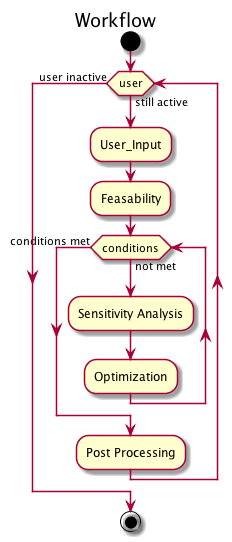
\includegraphics[scale=.5]{IMSM_Workflow.png}\end{center}

\subsection{Feasibility}
	\begin{enumerate}
		\item 
	\end{enumerate}

\subsection{Sensitivity Analysis}
	\begin{enumerate}
		\item
	\end{enumerate}

\subsection{Optimization}
	\begin{enumerate}
		\item
	\end{enumerate}

		
\section{Computational Experiments}
	\begin{enumerate}

		\item Case Studies
		
		\item Relaxation and Creep
		
	\end{enumerate}
	
	
		
\section{Summary and Future Work}
	\begin{enumerate}
	
		
		
		\item Computational Inefficiencies 
				
		\item 
		
		\item 
		
		\item 
		
		\item 
		
	\end{enumerate}
	
	\section{References}
		

	\end{document}
